%%% Local Variables: 
%%% mode: latex
%%% TeX-master: t
%%% End: 
\documentclass{article}
\usepackage{../tex/mysty}
\begin{document}
 
\maketitlepage{Societal Impact Report}{Ginger Tsai}
 
\setcounter{tocdepth}{2}
\tableofcontents
\newpage
% \listoftables
% \listoffigures
% \newpage
 
 
\section*{Executive Summary}
\label{sec:exec-summary}
 
Today's leading ophthalmological research focuses on precise
measurements of the eye, particularly in regard to myopia, in order to
determine genetic factors of the disease and its implications on gross
eye shape. Current measurement methods such as MRI and CT have proved
insufficient, facing trade-offs between cost, resolution, speed, and
physical complexity of machines. Therefore, the team has proposed a
high-resolution scanning device that provides a three-dimensional
reconstruction of gross eye shape using a vertically translating LED
micrometer in conjunction with a rotary motor and framework, linear
encoder, and linear actuator controlled by a data acquisition board.

Five potential impacts the device may have on society are
presented. Economically, the device will aid researchers of
ophthalmology, paleontology, and mechanical engineering by providing a
long-term cost and time saving tool with which to conduct
measurements. Environmentally, the manufacture, use, and disposal of the device
shall have a minimal impact due to optimizations available at
production low volume. The
ethical implications include a minimal likelihood chance of abuse of
genetic information, though it's consideration is important. The device faces
little to no regulation by the Food and Drug Administration and local
research facilities. In general, the device benefits society by
providing a tool which enables researchers to discover new treatments
and advance ophthalmological science while having minimal negative
impact on society or the environment.



% It's actually 313 words now, so --- booyah! -J

\newpage
 
  
\section{Introduction}
\label{sec:Introduction}
 
The cutting edge of ophthalmological research is focused on extremely
precise measurements of the eye, as research suggests a strong
connection between gross anatomical shape and eye health and
function. Particularly, new research is interested in precision
measurement of the exact exterior shape of the
eye\cite{atchison04,zhou99:genes,zhou99:models,guggenheim04,wallman04}. While
historically eye shape was parametrized by three axial lengths, the
anterior-posterior (AP) axis, the nasal-temporal (NT) axis, and the
superior-inferior (SI) axis, new studies are interested in non-linear,
higher-order parametrizations involving sphericity or even elliptical
properties of surface splines at any location on the eye.
 
An example domain for this research is the investigation of the
genetic factors involved in myopia, which is thought to be a symptom
of greater changes to overall eye shape \cite{atchison04}. Myopia,
which has a 25\% prevalence in western cultures and nearly 80\%
prevalence in some Asian populations\cite{rajan98}, is an extremely
common disease impacting eye function and focus. It is well-known to
be caused by environmental factors such as sustained near-viewing, but
is also increasingly shown to also have a genetic
correlate\cite{zhou99:genes,zhou99:models,schmucker04}. Studies of the
interaction of genetic factors with eye shape seek to determine both
ultimate and developmental genetic effects which result in myopic
eyes. Since the symptoms of myopia are directly caused by
over-extension of the AP axis, leading to a focal point that resides
within the cavity of the eye instead of at the sensitive retinal well,
these researchers are first interested in accurate measurement of the
AP axis\cite{wallman04}, but want to consider more sophisticated
deformations as in the NT and SI axes to truly understand the effect
of genetics on the development of a myopic eye\cite{schaeffel04} and
thus of gross eye shape \cite{atchison04}.
 
In order to perform such genetic analysis, much of this research is
carried out on mouse animal models due to availability, ease of
genetic manipulation, and
affordability\cite{schaeffel04}. Unfortunately, this means that the
observations must be made on mouse eyes, which range between 1.5 to 4
millimeters in diameter. At this size, affective anatomical
deformations occur at resolutions of 5 microns. Current research
methods include laborious, error-prone, unrepeatable manual
micrometry\cite{wallman04}; expensive and low-resolution MRI/PET
imaging\cite{atchison04}; error-inducing histological
sectioning\cite{schaeffel04}; or complex, inefficient optical
interferometry\cite{guggenheim04,schaeffel04}. A device capable of
three-dimensional imaging with high precision is thus needed to
facilitate progress of such ophthalmological research.
 
To meet these needs, the team has proposed a device which implements
complete three-dimensional reconstruction by scanning over the eye
with a laser-emitting diode (LED) micrometer. The device, pictured in
figure \ref{fig:schematic}, consists roughly of three parts including
an eye-actuating harness, the micrometer frame, and the computer
interface. The eye harness is the primary physical interaction point
for the user and thus enables easy replacement of specimens into the
device. Its purpose is to hold the eye and fix it rigidly for
acceleration without impacting the optical path for the micrometer. To
this end, it consists of a pair of reverse-action tweezers which are
fitted into a cylindrical cuvette filled with a high-viscosity methyl
cellulose buffer suspension. When the cuvette is inserted into the
frame of the device, it is placed against a corrective lens which
corrects for the optical distortion from the cylinder (not shown). The
harness then attaches to a motor supplemented by an angular encoder,
which can then accelerate the tube while keeping high-resolution data
on its current theta-position.
 
The frame itself holds the motors and the micrometer heads, which
consist of the receiver and transmitter. The heads are attached to a
microscope frame augmented with another motor/encoder pair to provide
linear articulation in the z-direction while maintaining
high-resolution position data. Finally, the data from the two encoders
and the micrometer is fed into a National Instruments Single-board
Reconfigurable Input Output device (sbRIO), which provides real-time
feedback and control while collecting data for online
reconstruction. The reconstruction algorithm itself is a modified
back-projection algorithm supplemented by cosine interpolation in the
z-direction.
 
In the process of designing and manufacturing a device, it is
important to consider the various impacts the device may have on
society throughout its lifetime. The team has analyzed five possible
impacts of the proposed device: demographics and economic impact,
medical ethics, public policy, and environmental concerns.
 
 
\subsection{Demographics and Economic Impact}
\label{sec:Demographics}
 
The target users of the device will be researchers in ophthalmology,
particularly those who conduct studies requiring precise measurements
of an eye. An estimated number of 500 researchers working at 70
medical research institutions will benefit from the device
\cite{Nickerson}, which will introduce new avenues to study the eye
while enabling researchers to conduct current research easier and
faster.  The improved performance supplied by
the device would translate into savings, in terms of both time and
money, for both researchers and organizations that fund them, such as
the National Institutes of Health (NIH). This in turn would allow money from the general public
and resources at research institutions to be invested in making
discoveries on more fronts, advancing scientific knowledge at a
greater rate.
 
Another demographic on which the device would have an impact is the
niche market of those who specialize in making optically precise
glassware. Two key components of the device are the optically precise
cuvette and corrective lens, both which would be purchased from
specific manufacturers. Additionally, the device could also
generalize to other use cases such as archaeologists with delicate
bone samples. These
populaces would benefit from use of the device similarly to the
ophthalmological scientists it is targetted at.

\subsection{Environmental Impact}
\label{sec:environment}
 
The device, intended for extended use in a controlled setting, is
posed to be highly environmentally conscientious. Due to the
relatively small number of potential buyers, the manufacture,
packaging, and shipping can all be optimized to minimize environmental
impact. The device itself produces little to no waste during operation
and presents nominal energy draw. Finally, should the user need to
dispose of the device due to failure or lifetime expiry, its modular
components such as the motor, encoder, and micrometer could easily be
repaired by a specialist or reused in new devices or in other
projects.
 
The team's proposed manufacturing methods need to serve a relatively
small consumer base of approximately 70 research labs in the US. At
this volume, the devices will likely be custom-fabricated using CNC
milling instead of more volume-dependent manufacturing methods such as
casting. Thus, the manufacturing process leaves behind a smaller
ecological footprint while outputting a product that is likely to last
through more cycles.

In order to continue with the green methods already proposed, the
device will be packaged using attractive, cheap recycled materials
such as recycled cardboard. Moreover, so long as the device can be
user-tested for designs which are intuitive and easy to use, a printed
manual need not be included in the packaging. Instead, directions to
an online manual will be provided, saving further packaging and
resource consumption.
 
During its lifetime of use, the device consumes very little
material. All pieces are high quality, robust, and often optically
precise, requiring that each component is cleaned and reused instead
of being disposed. While it is possible that parts such as the
mounting cuvette could shatter if mishandled, the consumer should take
care in reducing the frequency of this sort of waste, especially since
optically-precise cuvettes are expensive.
 
The proposed device therefore is well poised to cause minimal
environmental damage through its manufacture, sale, operation, and
disposal. The team supports this capability with a commitment to the
available environmentally friendly processes by erring on the
side of quality and re-usability.
 
 
\subsection{Medical Ethics}
\label{sec:blah-blah-blah}
 
% I had no idea what was going on here for a while

As with any research-oriented goal, the distant effects of proximal
successes are difficult to gauge. However, it is clear that this
device most immediately affects knowledge of the genetic factors in
eye development, especially abnormal, myopic eye development.

With any advance in genetics, there is concern for treatment,
identification, and policy-level decisions concerning those affected
by any genetic predispositions. For instance, the United States Air
Force, notorious for rejecting on valid grounds those without 20/20
vision, could foreseeably extend their recruitment programs to reject
those who have a high chance of developing myopia (or demanding that
they receive elective surgeries to correct for it). The proposed
device could be key in discovering and proving these genetic tests and
consequently in influencing national policy.

Use of the device by the untrained, uninformed general public may lead
to misinterpretation of eye shape deformities and to widespread
unethical abuse of genetic information in employment processes,
national policy, and general behavior. The device should therefore be
used either in research settings or in confidential settings for
medical purposes.  Even so, enabling people to more accurately predict
myopia is unlikely to cause much harm.  In the vast majority of cases,
myopia already has a non-invasive, popular treatment: common
eyeglasses. Additionally, as time goes forward it is likely that
surgical laser-corrective methods will both improve and drop in price,
making that an attractive option. Genetic causes of eye deformation
may even be affected \textit{post hoc} by treating the secondary steps
in the development of these diseases. All of these methods could gain
both in awareness, affordability, and availability from the research
enabled by the device.
 
To this end, our device is well in-line with the ethical principles of
today. Its deployment in confidential medical contexts is unlikely to
cause harm to people and instead may provide new opportunities to
reclaim ability that normally would be lost to ocular deformation.
 
 
\subsection{Public Policy}
\label{sec:Public Policy}
 
The device will not be regulated by the Food and Drug
Administration. It is not intended to diagnose, treat, mitigate, or
cure any disease, nor will it come into contact with live tissue in
any way; hence, it is not considered a medical device as defined in
the Federal Food, Drug, and Cosmetic Act (FFDCA) section 201(h)
\cite{fdaguidelines}. Also, since the device will not be used on live
tissues, there is little regulation necessary concerning the sterility
or the material properties of the device beyond possible biological
contamination from the dissected eyeball, whose treatment and disposal
is regulated by the local regulations of the research facility.  Even
though the LED micrometer of the device employs visible light, it is
minimally regulated by the FFDCA, as it can be classified as a Class I
laser product according to sections 1040.10, for it "does not permit
access during the operation to levels of laser radiation in excess of
the accessible emission limits" \cite{fdaguidelines}.
 
 
\section{Conclusion}
\label{sec:Conclusion}

In general, the device contributes to society in a beneficial
manner. It requires minimal regulation and leaves a minimal ecological
footprint, while serving as a cost- and time-saving long-term
investment for ophthalmological researchers and possibly for
researchers in paleontology and mechanical engineering.  Though the
use of the device must be confined to confidential medical and
research contexts, the device presents a novel influence on national
policy and on further treatment for myopia or other genetic causes of
eye deformation.

\section{Addendums}
\label{sec:addendums}

\subsection{Figures}
\label{sec:figures}

\begin{figure}[H]
  \centering
  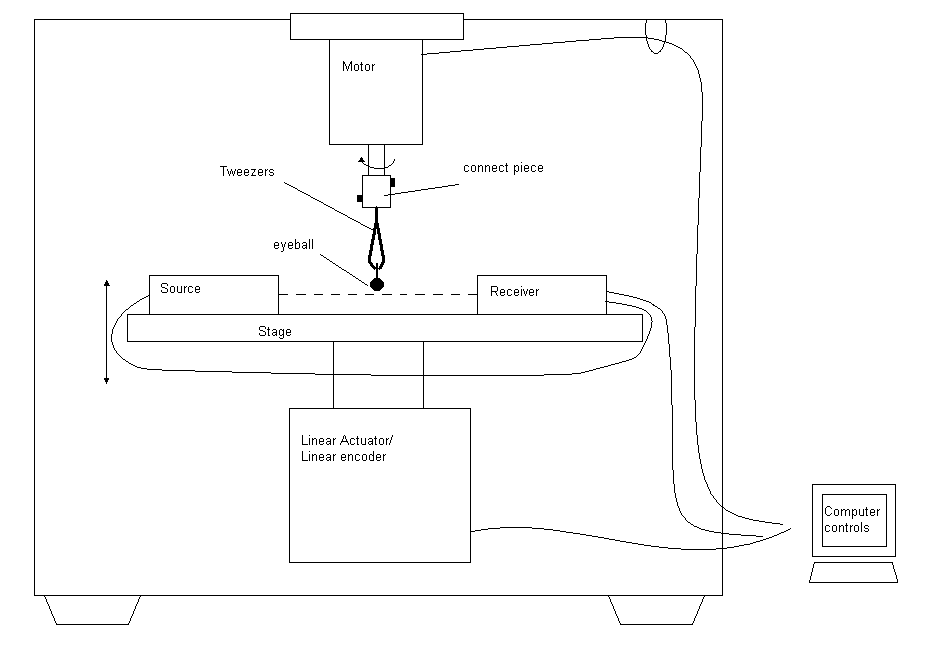
\includegraphics[width=\linewidth]{../img/schematic1}
  \figcaption{\textbf{Schematic of the Prototype:} This figure
    illustrates the physical organization of the various components of
    the design within an enclosed framework. Each component is
    labeled. }
  \label{fig:schematic}
\end{figure}
 
\newpage
\addcontentsline{toc}{section}{References}
\bibliographystyle{unsrt}
\bibliography{../tex/bibl}
 
\end{document}
 
